\documentclass[12pt,oneside]{book}
\usepackage{geometry}                		% See geometry.pdf to learn the layout options. There are lots.
\geometry{a4paper}                   			% ... or a4paper or a5paper or ... 
%\geometry{landscape}                		% Activate for for rotated page geometry
%\usepackage[parfill]{parskip}    		% Activate to begin paragraphs with an empty line rather than an indent
\usepackage{graphicx}				% Use pdf, png, jpg, or epsß with pdflatex; use eps in DVI mode
								% TeX will automatically convert eps --> pdf in pdflatex		
\usepackage{amssymb}

\usepackage[spanish]{babel}			% Permite que partes automáticas del documento aparezcan en castellano.
\usepackage[utf8]{inputenc}			% Permite escribir tildes y otros caracteres directamente en el .tex
\usepackage[T1]{fontenc}				% Asegura que el documento resultante use caracteres de una fuente apropiada.

\usepackage{hyperref}				% Permite poner urls y links dentro del documento

\title{Mi Juego Favorito}
\author{Rubén Carvajal\\
\and
Cesar Madrid\\
\and
Jefferson Rivera}
%\date{}							% Activate to display a given date or no date

\begin{document}
\maketitle
\tableofcontents


\chapter{Introducción}
El libro a continuación es creado como una herramienta para el desarrollo de habilidades de edición colaborativa de documentos de texto plano. La herramienta que habilita dicha colaboración, en este taller, es Git pero podría ser reemplazada por otros sistemas de versionamiento.

\chapter{Los Juegos}

\section{Arcane Legends}

\begin{figure}[htbp]
\begin{center}
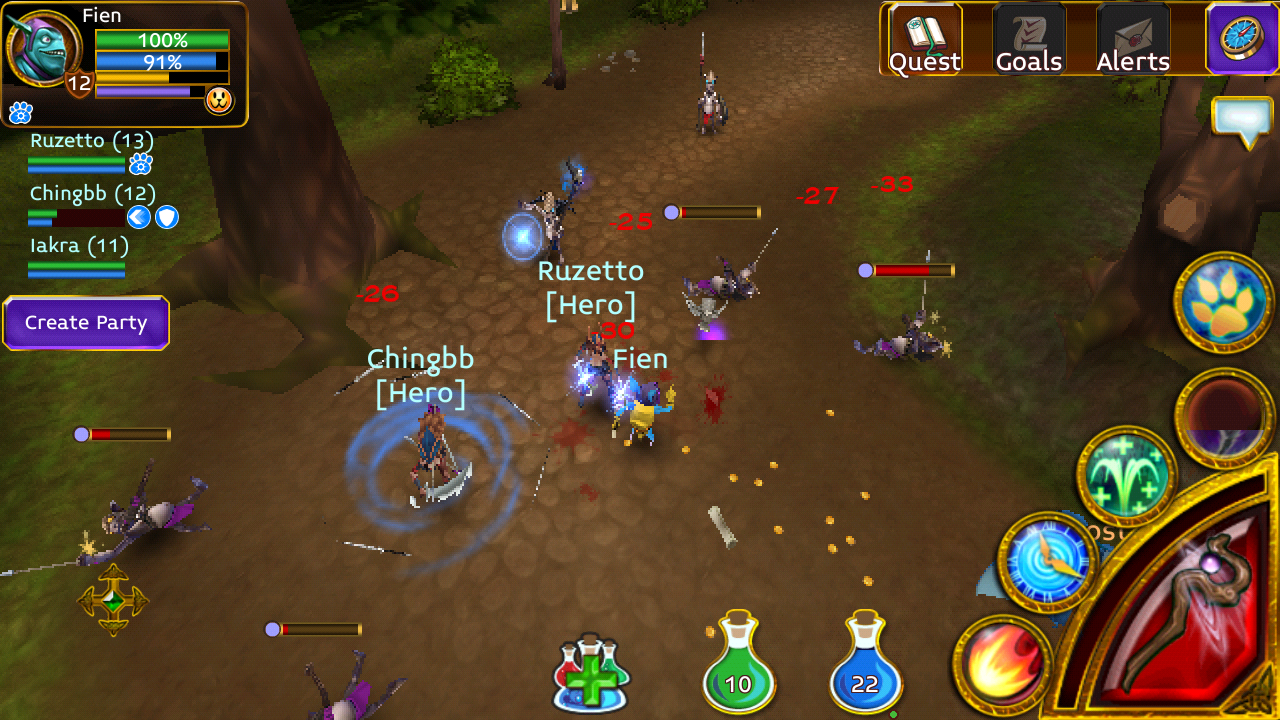
\includegraphics[width=.60\textwidth]{./imagenes/arcanelegends.png}
\caption{Arcane Legends}
\label{Arcane Legends}
\end{center}
\end{figure}
Arcane Legends\footnote{\url{http://www.arcanelegendsgame.com/}} es un juego para plataformas moviles  de tipo MMORPG totalmente gratuito en el que podrás combatir en modo cooperativo con otros usuarios de la red y derrotar el mal que encontrarás por todas partes. El personaje que elijas marcará tu personalidad y puedes elegir tres tipos, un pícaro, un mago o un guerrero. Una de las mejores características del juego se basa en un compañero animal que llevas a tu lado y que podrás mandar a tu antojo para que te ayude en la lucha. Además podrás hacerle evolucionar y añadirle poderes extra.

\subsubsection{¿Por qué es uno de mis juegos favoritos?}
\begin{itemize}
\item[César Madrid].
\end{itemize}

\section{Crysis 2}

\begin{figure}[htbp]
\begin{center}
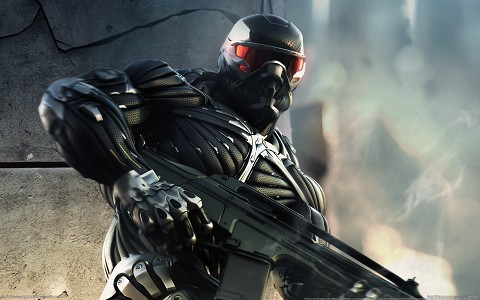
\includegraphics[width=.60\textwidth]{./imagenes/crysis2.jpg}
\caption{Crysis 2}
\label{Crysis 2}
\end{center}
\end{figure}
Crysis 2 \footnote{\url{http://www.ea.com/es/crysis2}} es un videojuego de disparos en primera persona desarrollado por la empresa Crytek y distribuido por Electronic Arts. Fue publicado en marzo de 2011 para PC, Xbox 360 y PlayStation 3. Es la secuela de Crysis y el primer videojuego en usar el motor CryEngine 3 desarrollado por Crytek también.

\subsubsection{¿Por qué es uno de mis juegos favoritos?}
\begin{itemize}
\item[Rubén Carvajal] La esencia del juego es magnifica, la historia consigue atraparte con su argumento futurístico.
Uno puede jugarlo a su manera, dependiendo del escenario habrán momentos en que te guste más pasar a todos descargando todo tu arcenal de armas, o momentos en que lo que sirva más sea utilizar las multiples opciones del traje y el sigilo.
La jugabilidad y los gráficos son de altísima calidad, las opciones de camuflaje y el entorno en el que se desarrolla el juego son particularidades destacables.

El sonido de cada ambiente está bien trabajado, e incluso tenemos opciones gráficas en 3D, cosas que hacen de este un exelente juego.
\end{itemize}


\chapter{Conclusiones}
Cuales juegos fueron más populares y un breve razonamiento del porqué.

\end{document}  
